\documentclass[a4paper]{book}
\usepackage{makeidx}
\usepackage{natbib}
\usepackage{graphicx}
\usepackage{multicol}
\usepackage{float}
\usepackage{listings}
\usepackage{color}
\usepackage{ifthen}
\usepackage[table]{xcolor}
\usepackage{textcomp}
\usepackage{alltt}
\usepackage{ifpdf}
\ifpdf
\usepackage[pdftex,
            pagebackref=true,
            colorlinks=true,
            linkcolor=blue,
            unicode
           ]{hyperref}
\else
\usepackage[ps2pdf,
            pagebackref=true,
            colorlinks=true,
            linkcolor=blue,
            unicode
           ]{hyperref}
\usepackage{pspicture}
\fi
\usepackage[utf8]{inputenc}
\usepackage{polski}
\usepackage[T1]{fontenc}

\usepackage{mathptmx}
\usepackage[scaled=.90]{helvet}
\usepackage{courier}
\usepackage{sectsty}
\usepackage[titles]{tocloft}
\usepackage{doxygen}
\lstset{language=C++,inputencoding=utf8,basicstyle=\footnotesize,breaklines=true,breakatwhitespace=true,tabsize=8,numbers=left }
\makeindex
\setcounter{tocdepth}{3}
\renewcommand{\footrulewidth}{0.4pt}
\renewcommand{\familydefault}{\sfdefault}
\hfuzz=15pt
\setlength{\emergencystretch}{15pt}
\hbadness=750
\tolerance=750
\begin{document}
\hypersetup{pageanchor=false,citecolor=blue}
\begin{titlepage}
\vspace*{7cm}
\begin{center}
{\Large \-Lab6 }\\
\vspace*{1cm}
{\large \-Wygenerowano przez Doxygen 1.7.6.1}\\
\vspace*{0.5cm}
{\small Tue Apr 22 2014 16:34:33}\\
\end{center}
\end{titlepage}
\clearemptydoublepage
\pagenumbering{roman}
\tableofcontents
\clearemptydoublepage
\pagenumbering{arabic}
\hypersetup{pageanchor=true,citecolor=blue}
\chapter{\-Struktura katalogów}
\section{\-Katalogi}
\-Ta struktura katalogów jest posortowana jest z grubsza, choć nie całkowicie, alfabetycznie\-:\begin{DoxyCompactList}
\item \contentsline{section}{prj}{\pageref{dir_9f92f53661fd78c561fa1672d6c740cd}}{}
\end{DoxyCompactList}

\chapter{\-Indeks klas}
\section{\-Lista klas}
\-Tutaj znajdują się klasy, struktury, unie i interfejsy wraz z ich krótkimi opisami\-:\begin{DoxyCompactList}
\item\contentsline{section}{\hyperlink{class_drzewo}{\-Drzewo$<$ K, W $>$} \\*\-Modeluje pojecie drzewa binarnego. \-Jego atrybutem jest klasa \hyperlink{class_wezel}{\-Wezel} }{\pageref{class_drzewo}}{}
\item\contentsline{section}{\hyperlink{class_para}{\-Para$<$ K, W $>$} \\*\-Modeluje pojecie pary. \-Jej atrybutem sa pola zawierajace klucz i wartosci }{\pageref{class_para}}{}
\item\contentsline{section}{\hyperlink{class_tablica}{\-Tablica$<$ K, W $>$} \\*\-Modeluje pojecie tablicy z haszowaniem. \-Klasa modeluje pojecie tablicy z haszowaniem. \-Jej atrybutami sa pola\-: klucz i wartosc }{\pageref{class_tablica}}{}
\item\contentsline{section}{\hyperlink{class_wezel}{\-Wezel$<$ K, W $>$} \\*\-Modeluje pojecie wezla. \-Jego atrybutem jest klasa \hyperlink{class_para}{\-Para} }{\pageref{class_wezel}}{}
\end{DoxyCompactList}

\chapter{\-Indeks plików}
\section{\-Lista plików}
\-Tutaj znajduje się lista wszystkich plików z ich krótkimi opisami\-:\begin{DoxyCompactList}
\item\contentsline{section}{\hyperlink{main_8cpp}{main.\-cpp} \\*\-Plik zawiera glowna funkcje programu }{\pageref{main_8cpp}}{}
\item\contentsline{section}{\hyperlink{simplex_8cpp}{simplex.\-cpp} \\*\-Definicje poszczegolnych funkcji dla klasy \hyperlink{class_simplex}{\-Simplex} }{\pageref{simplex_8cpp}}{}
\item\contentsline{section}{\hyperlink{simplex_8h}{simplex.\-h} \\*\-Plik naglowkowy klasy \hyperlink{class_simplex}{\-Simplex} }{\pageref{simplex_8h}}{}
\end{DoxyCompactList}

\chapter{\-Dokumentacja katalogów}
\hypertarget{dir_269ca723671743fe5d05b443db073096}{\section{\-Dokumentacja katalogu /home/martyna/pamsi2/lab6/prj/inc/}
\label{dir_269ca723671743fe5d05b443db073096}\index{\-Dokumentacja katalogu /home/martyna/pamsi2/lab6/prj/inc/@{\-Dokumentacja katalogu /home/martyna/pamsi2/lab6/prj/inc/}}
}
\-Directory dependency graph for /home/martyna/pamsi2/lab6/prj/inc/\-:
\nopagebreak
\begin{figure}[H]
\begin{center}
\leavevmode
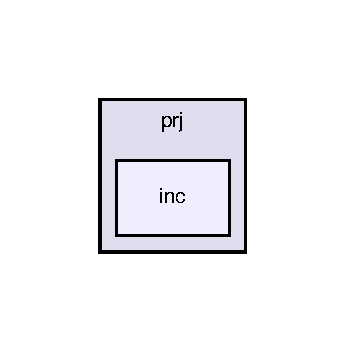
\includegraphics[width=166pt]{dir_269ca723671743fe5d05b443db073096_dep}
\end{center}
\end{figure}
\subsection*{\-Pliki}
\begin{DoxyCompactItemize}
\item 
plik \hyperlink{_drzewo_8h}{\-Drzewo.\-h}
\item 
plik \hyperlink{_para_8h}{\-Para.\-h}
\item 
plik \hyperlink{_tablica_8h}{\-Tablica.\-h}
\item 
plik \hyperlink{_wezel_8h}{\-Wezel.\-h}
\end{DoxyCompactItemize}

\hypertarget{dir_ec6420f7dab0d6dc90d0aeca5797a0bf}{\section{\-Dokumentacja katalogu /home/martyna/pamsi2/lab6/prj/}
\label{dir_ec6420f7dab0d6dc90d0aeca5797a0bf}\index{\-Dokumentacja katalogu /home/martyna/pamsi2/lab6/prj/@{\-Dokumentacja katalogu /home/martyna/pamsi2/lab6/prj/}}
}
\-Directory dependency graph for /home/martyna/pamsi2/lab6/prj/\-:
\nopagebreak
\begin{figure}[H]
\begin{center}
\leavevmode
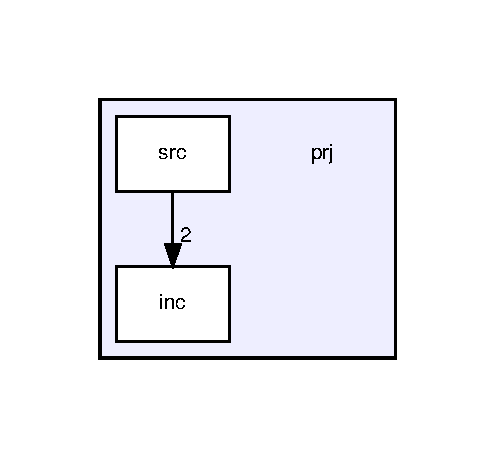
\includegraphics[width=238pt]{dir_ec6420f7dab0d6dc90d0aeca5797a0bf_dep}
\end{center}
\end{figure}
\subsection*{\-Katalogi}
\begin{DoxyCompactItemize}
\item 
katalog \hyperlink{dir_269ca723671743fe5d05b443db073096}{inc}
\item 
katalog \hyperlink{dir_9fd0c07b1190a8b7276b0ba7a5123eb1}{src}
\end{DoxyCompactItemize}

\hypertarget{dir_9fd0c07b1190a8b7276b0ba7a5123eb1}{\section{\-Dokumentacja katalogu /home/martyna/pamsi2/lab6/prj/src/}
\label{dir_9fd0c07b1190a8b7276b0ba7a5123eb1}\index{\-Dokumentacja katalogu /home/martyna/pamsi2/lab6/prj/src/@{\-Dokumentacja katalogu /home/martyna/pamsi2/lab6/prj/src/}}
}
\-Directory dependency graph for /home/martyna/pamsi2/lab6/prj/src/\-:
\nopagebreak
\begin{figure}[H]
\begin{center}
\leavevmode
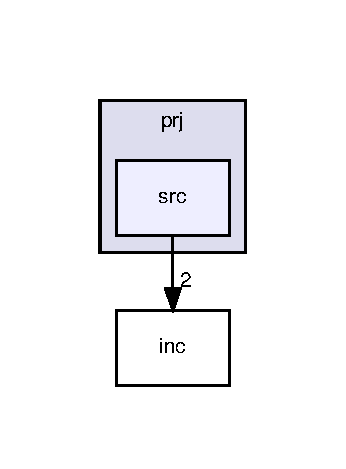
\includegraphics[width=166pt]{dir_9fd0c07b1190a8b7276b0ba7a5123eb1_dep}
\end{center}
\end{figure}
\subsection*{\-Pliki}
\begin{DoxyCompactItemize}
\item 
plik \hyperlink{_main_8cpp}{\-Main.\-cpp}
\item 
plik \hyperlink{_para_8cpp}{\-Para.\-cpp}
\end{DoxyCompactItemize}

\chapter{\-Dokumentacja klas}
\hypertarget{class_drzewo}{\section{\-Dokumentacja szablonu klasy \-Drzewo$<$ \-K, \-W $>$}
\label{class_drzewo}\index{\-Drzewo$<$ K, W $>$@{\-Drzewo$<$ K, W $>$}}
}


{\ttfamily \#include $<$\-Drzewo.\-h$>$}

\subsection*{\-Metody publiczne}
\begin{DoxyCompactItemize}
\item 
\hyperlink{class_drzewo_a123b6a71eed621cac3eaf0be8832472f}{\-Drzewo} ()
\item 
\hyperlink{class_drzewo_af342485cb51b160c303a57fada508642}{$\sim$\-Drzewo} ()
\item 
\hyperlink{class_drzewo_a69255eed324949a2e0dbcda0ea5bd011}{\-Drzewo} (const \hyperlink{class_drzewo}{\-Drzewo} \&drzewo)
\item 
void \hyperlink{class_drzewo_a81d5e253a86cc6e42ab011d3e2157d1a}{dodaj} (\-K klucz, \-W wartosc)
\item 
\-W \hyperlink{class_drzewo_add8d5fe17b7552b3d494fa5b9c49ce6b}{pobierz\-Wartosc} (\-K klucz)
\item 
void \hyperlink{class_drzewo_a7ff767a6ea6bc9c418d1fb24ed0d6276}{usun} (\-K klucz)
\item 
\hyperlink{class_wezel}{\-Wezel}$<$ \-K, \-W $>$ $\ast$\& \hyperlink{class_drzewo_a5e331e1a37bf317c2742b94a34e93b2e}{nastepnik} (\hyperlink{class_wezel}{\-Wezel}$<$ \-K, \-W $>$ $\ast$\&wezel, \hyperlink{class_wezel}{\-Wezel}$<$ \-K, \-W $>$ $\ast$\&us)
\end{DoxyCompactItemize}
\subsection*{\-Metody prywatne}
\begin{DoxyCompactItemize}
\item 
void \hyperlink{class_drzewo_af32cbb347cb334efa59ca8bf83f0c343}{dodaj} (\-K klucz, \-W wartosc, \hyperlink{class_wezel}{\-Wezel}$<$ \-K, \-W $>$ $\ast$\&wsk)
\item 
\hyperlink{class_wezel}{\-Wezel}$<$ \-K, \-W $>$ $\ast$\& \hyperlink{class_drzewo_a0353214a4242185bd700f361246ad928}{usun} (\-K klucz, \hyperlink{class_wezel}{\-Wezel}$<$ \-K, \-W $>$ $\ast$\&wezel)
\end{DoxyCompactItemize}
\subsection*{\-Atrybuty prywatne}
\begin{DoxyCompactItemize}
\item 
\hyperlink{class_wezel}{\-Wezel}$<$ \-K, \-W $>$ $\ast$ \hyperlink{class_drzewo_a98a51a2f29c2084a3a3c393b62148511}{korzen}
\item 
int \hyperlink{class_drzewo_aced92fc2774839454279308ef420d6d4}{liczba\-Elementow}
\end{DoxyCompactItemize}


\subsection{\-Opis szczegółowy}
\subsubsection*{template$<$typename \-K, typename \-W$>$class Drzewo$<$ K, W $>$}

\-Modeluje pojecie drzewa binarnego. \-Jego atrybutem jest klasa \hyperlink{class_wezel}{\-Wezel}. 

\subsection{\-Dokumentacja konstruktora i destruktora}
\hypertarget{class_drzewo_a123b6a71eed621cac3eaf0be8832472f}{\index{\-Drzewo@{\-Drzewo}!\-Drzewo@{\-Drzewo}}
\index{\-Drzewo@{\-Drzewo}!Drzewo@{\-Drzewo}}
\subsubsection[{\-Drzewo}]{\setlength{\rightskip}{0pt plus 5cm}template$<$typename K , typename W $>$ {\bf \-Drzewo}$<$ \-K, \-W $>$\-::{\bf \-Drzewo} (
\begin{DoxyParamCaption}
{}
\end{DoxyParamCaption}
)}}\label{class_drzewo_a123b6a71eed621cac3eaf0be8832472f}


\-Konstruktor klasy \hyperlink{class_drzewo}{\-Drzewo}. \-Bezargumentowy. 

\hypertarget{class_drzewo_af342485cb51b160c303a57fada508642}{\index{\-Drzewo@{\-Drzewo}!$\sim$\-Drzewo@{$\sim$\-Drzewo}}
\index{$\sim$\-Drzewo@{$\sim$\-Drzewo}!Drzewo@{\-Drzewo}}
\subsubsection[{$\sim$\-Drzewo}]{\setlength{\rightskip}{0pt plus 5cm}template$<$typename K , typename W $>$ {\bf \-Drzewo}$<$ \-K, \-W $>$\-::$\sim${\bf \-Drzewo} (
\begin{DoxyParamCaption}
{}
\end{DoxyParamCaption}
)}}\label{class_drzewo_af342485cb51b160c303a57fada508642}


\-Destruktor klasy \hyperlink{class_drzewo}{\-Drzewo}. \-Czysci pamiec po obiekcie. 

\hypertarget{class_drzewo_a69255eed324949a2e0dbcda0ea5bd011}{\index{\-Drzewo@{\-Drzewo}!\-Drzewo@{\-Drzewo}}
\index{\-Drzewo@{\-Drzewo}!Drzewo@{\-Drzewo}}
\subsubsection[{\-Drzewo}]{\setlength{\rightskip}{0pt plus 5cm}template$<$typename K , typename W $>$ {\bf \-Drzewo}$<$ \-K, \-W $>$\-::{\bf \-Drzewo} (
\begin{DoxyParamCaption}
\item[{const {\bf \-Drzewo}$<$ \-K, \-W $>$ \&}]{drzewo}
\end{DoxyParamCaption}
)}}\label{class_drzewo_a69255eed324949a2e0dbcda0ea5bd011}


\-Konstruktor kopiujacy klasy \hyperlink{class_drzewo}{\-Drzewo}. \-Kopiuje obiekt. 



\subsection{\-Dokumentacja funkcji składowych}
\hypertarget{class_drzewo_af32cbb347cb334efa59ca8bf83f0c343}{\index{\-Drzewo@{\-Drzewo}!dodaj@{dodaj}}
\index{dodaj@{dodaj}!Drzewo@{\-Drzewo}}
\subsubsection[{dodaj}]{\setlength{\rightskip}{0pt plus 5cm}template$<$typename K , typename W $>$ void {\bf \-Drzewo}$<$ \-K, \-W $>$\-::{\bf dodaj} (
\begin{DoxyParamCaption}
\item[{\-K}]{klucz, }
\item[{\-W}]{wartosc, }
\item[{{\bf \-Wezel}$<$ \-K, \-W $>$ $\ast$\&}]{wsk}
\end{DoxyParamCaption}
)\hspace{0.3cm}{\ttfamily  \mbox{[}private\mbox{]}}}}\label{class_drzewo_af32cbb347cb334efa59ca8bf83f0c343}


\-Funkcja dodaj. \-Dodaje wezel do drzewa. 



\-Oto graf wywoływań tej funkcji\-:
\nopagebreak
\begin{figure}[H]
\begin{center}
\leavevmode
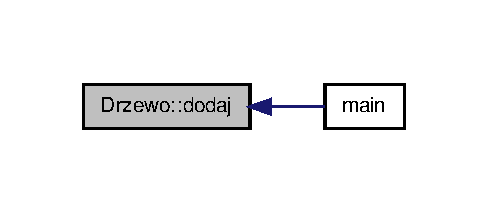
\includegraphics[width=234pt]{class_drzewo_af32cbb347cb334efa59ca8bf83f0c343_icgraph}
\end{center}
\end{figure}


\hypertarget{class_drzewo_a81d5e253a86cc6e42ab011d3e2157d1a}{\index{\-Drzewo@{\-Drzewo}!dodaj@{dodaj}}
\index{dodaj@{dodaj}!Drzewo@{\-Drzewo}}
\subsubsection[{dodaj}]{\setlength{\rightskip}{0pt plus 5cm}template$<$typename K , typename W $>$ void {\bf \-Drzewo}$<$ \-K, \-W $>$\-::{\bf dodaj} (
\begin{DoxyParamCaption}
\item[{\-K}]{klucz, }
\item[{\-W}]{wartosc}
\end{DoxyParamCaption}
)}}\label{class_drzewo_a81d5e253a86cc6e42ab011d3e2157d1a}


\-Funkcja dodaj. \-Dodaje wezel do drzewa. 

\hypertarget{class_drzewo_a5e331e1a37bf317c2742b94a34e93b2e}{\index{\-Drzewo@{\-Drzewo}!nastepnik@{nastepnik}}
\index{nastepnik@{nastepnik}!Drzewo@{\-Drzewo}}
\subsubsection[{nastepnik}]{\setlength{\rightskip}{0pt plus 5cm}template$<$typename K , typename W $>$ {\bf \-Wezel}$<$ \-K, \-W $>$ $\ast$\& {\bf \-Drzewo}$<$ \-K, \-W $>$\-::{\bf nastepnik} (
\begin{DoxyParamCaption}
\item[{{\bf \-Wezel}$<$ \-K, \-W $>$ $\ast$\&}]{wezel, }
\item[{{\bf \-Wezel}$<$ \-K, \-W $>$ $\ast$\&}]{us}
\end{DoxyParamCaption}
)}}\label{class_drzewo_a5e331e1a37bf317c2742b94a34e93b2e}


\-Funkcja nastepnik. \-Wyszukuje i wstawia w odpowiednie miejsce nastepnika. 

\hypertarget{class_drzewo_add8d5fe17b7552b3d494fa5b9c49ce6b}{\index{\-Drzewo@{\-Drzewo}!pobierz\-Wartosc@{pobierz\-Wartosc}}
\index{pobierz\-Wartosc@{pobierz\-Wartosc}!Drzewo@{\-Drzewo}}
\subsubsection[{pobierz\-Wartosc}]{\setlength{\rightskip}{0pt plus 5cm}template$<$typename K , typename W $>$ \-W {\bf \-Drzewo}$<$ \-K, \-W $>$\-::{\bf pobierz\-Wartosc} (
\begin{DoxyParamCaption}
\item[{\-K}]{klucz}
\end{DoxyParamCaption}
)}}\label{class_drzewo_add8d5fe17b7552b3d494fa5b9c49ce6b}


\-Funkcja pobierz\-Wartosc. \-Zwraca wartosc przypisana do klucza. 



\-Oto graf wywoływań tej funkcji\-:\nopagebreak
\begin{figure}[H]
\begin{center}
\leavevmode
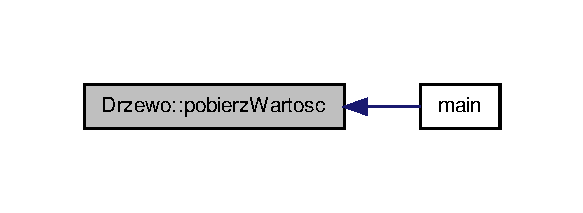
\includegraphics[width=280pt]{class_drzewo_add8d5fe17b7552b3d494fa5b9c49ce6b_icgraph}
\end{center}
\end{figure}


\hypertarget{class_drzewo_a0353214a4242185bd700f361246ad928}{\index{\-Drzewo@{\-Drzewo}!usun@{usun}}
\index{usun@{usun}!Drzewo@{\-Drzewo}}
\subsubsection[{usun}]{\setlength{\rightskip}{0pt plus 5cm}template$<$typename K , typename W $>$ {\bf \-Wezel}$<$ \-K, \-W $>$ $\ast$\& {\bf \-Drzewo}$<$ \-K, \-W $>$\-::{\bf usun} (
\begin{DoxyParamCaption}
\item[{\-K}]{klucz, }
\item[{{\bf \-Wezel}$<$ \-K, \-W $>$ $\ast$\&}]{wezel}
\end{DoxyParamCaption}
)\hspace{0.3cm}{\ttfamily  \mbox{[}private\mbox{]}}}}\label{class_drzewo_a0353214a4242185bd700f361246ad928}


\-Funkcja usun. \-Usuwa wezel z drzewa. 



\-Oto graf wywoływań tej funkcji\-:
\nopagebreak
\begin{figure}[H]
\begin{center}
\leavevmode
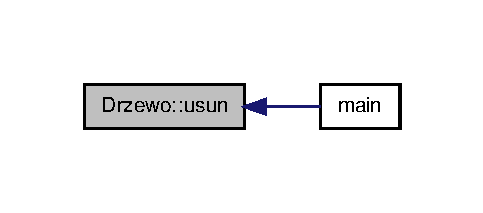
\includegraphics[width=232pt]{class_drzewo_a0353214a4242185bd700f361246ad928_icgraph}
\end{center}
\end{figure}


\hypertarget{class_drzewo_a7ff767a6ea6bc9c418d1fb24ed0d6276}{\index{\-Drzewo@{\-Drzewo}!usun@{usun}}
\index{usun@{usun}!Drzewo@{\-Drzewo}}
\subsubsection[{usun}]{\setlength{\rightskip}{0pt plus 5cm}template$<$typename K , typename W $>$ void {\bf \-Drzewo}$<$ \-K, \-W $>$\-::{\bf usun} (
\begin{DoxyParamCaption}
\item[{\-K}]{klucz}
\end{DoxyParamCaption}
)}}\label{class_drzewo_a7ff767a6ea6bc9c418d1fb24ed0d6276}


\-Funkcja usun. \-Usuwa wezel z drzewa. 



\subsection{\-Dokumentacja atrybutów składowych}
\hypertarget{class_drzewo_a98a51a2f29c2084a3a3c393b62148511}{\index{\-Drzewo@{\-Drzewo}!korzen@{korzen}}
\index{korzen@{korzen}!Drzewo@{\-Drzewo}}
\subsubsection[{korzen}]{\setlength{\rightskip}{0pt plus 5cm}template$<$typename \-K, typename \-W$>$ {\bf \-Wezel}$<$\-K,\-W$>$$\ast$ {\bf \-Drzewo}$<$ \-K, \-W $>$\-::{\bf korzen}\hspace{0.3cm}{\ttfamily  \mbox{[}private\mbox{]}}}}\label{class_drzewo_a98a51a2f29c2084a3a3c393b62148511}


\-Poczatkowy element drzewa -\/ korzen. 

\hypertarget{class_drzewo_aced92fc2774839454279308ef420d6d4}{\index{\-Drzewo@{\-Drzewo}!liczba\-Elementow@{liczba\-Elementow}}
\index{liczba\-Elementow@{liczba\-Elementow}!Drzewo@{\-Drzewo}}
\subsubsection[{liczba\-Elementow}]{\setlength{\rightskip}{0pt plus 5cm}template$<$typename \-K, typename \-W$>$ int {\bf \-Drzewo}$<$ \-K, \-W $>$\-::{\bf liczba\-Elementow}\hspace{0.3cm}{\ttfamily  \mbox{[}private\mbox{]}}}}\label{class_drzewo_aced92fc2774839454279308ef420d6d4}


\-Obecna liczba elementow w tablicy. 



\-Dokumentacja dla tej klasy została wygenerowana z pliku\-:\begin{DoxyCompactItemize}
\item 
\hyperlink{_drzewo_8h}{\-Drzewo.\-h}\end{DoxyCompactItemize}

\hypertarget{class_para}{\section{\-Dokumentacja szablonu klasy \-Para$<$ \-K, \-W $>$}
\label{class_para}\index{\-Para$<$ K, W $>$@{\-Para$<$ K, W $>$}}
}


{\ttfamily \#include $<$\-Para.\-h$>$}

\subsection*{\-Metody publiczne}
\begin{DoxyCompactItemize}
\item 
\hyperlink{class_para_a8ed1c319f0eaa368ce1c684bff7019ac}{\-Para} (\-K \hyperlink{class_para_a1cf136d1d7c4c7fca4662a04276d744a}{klucz}, \-W \hyperlink{class_para_a942bf7c31ea059ed0cfe1ac41bb21d6b}{wartosc})
\item 
\hyperlink{class_para_a7a6579dbfcb3730202886e82bc9fd345}{\-Para} (void)
\item 
\hyperlink{class_para_a18e9559206df6774b2c0e17ce373f2ac}{$\sim$\-Para} (void)
\item 
\hyperlink{class_para_a0229fba16ccbc9e3019d6db3cf9a6d51}{\-Para} (const \hyperlink{class_para}{\-Para} \&para)
\item 
\-K \& \hyperlink{class_para_a2290aed234696b309e979ae269e142ff}{pobierz\-Klucz} (void) const 
\item 
\-W \& \hyperlink{class_para_a3081579446074d32816e0299743208ca}{pobierz\-Wartosc} (void) const 
\item 
void \hyperlink{class_para_a5582293e44ba99f062dcb9fa8e99beaf}{ustaw\-Klucz} (\-K \hyperlink{class_para_a1cf136d1d7c4c7fca4662a04276d744a}{klucz})
\item 
void \hyperlink{class_para_aee0473cc5204fb4b86b2698c0bd7d150}{ustaw\-Wartosc} (\-W \hyperlink{class_para_a942bf7c31ea059ed0cfe1ac41bb21d6b}{wartosc})
\end{DoxyCompactItemize}
\subsection*{\-Atrybuty prywatne}
\begin{DoxyCompactItemize}
\item 
\-K $\ast$ \hyperlink{class_para_a1cf136d1d7c4c7fca4662a04276d744a}{klucz}
\item 
\-W $\ast$ \hyperlink{class_para_a942bf7c31ea059ed0cfe1ac41bb21d6b}{wartosc}
\end{DoxyCompactItemize}


\subsection{\-Opis szczegółowy}
\subsubsection*{template$<$typename \-K, typename \-W$>$class Para$<$ K, W $>$}

\-Modeluje pojecie pary. \-Jej atrybutem sa pola zawierajace klucz i wartosci. 

\subsection{\-Dokumentacja konstruktora i destruktora}
\hypertarget{class_para_a8ed1c319f0eaa368ce1c684bff7019ac}{\index{\-Para@{\-Para}!\-Para@{\-Para}}
\index{\-Para@{\-Para}!Para@{\-Para}}
\subsubsection[{\-Para}]{\setlength{\rightskip}{0pt plus 5cm}template$<$typename K , typename W $>$ {\bf \-Para}$<$ \-K, \-W $>$\-::{\bf \-Para} (
\begin{DoxyParamCaption}
\item[{\-K}]{klucz, }
\item[{\-W}]{wartosc}
\end{DoxyParamCaption}
)}}\label{class_para_a8ed1c319f0eaa368ce1c684bff7019ac}


\-Konstruktor klasy \hyperlink{class_para}{\-Para}. \-Jego argumentami sa klucz i wartosci. 

\hypertarget{class_para_a7a6579dbfcb3730202886e82bc9fd345}{\index{\-Para@{\-Para}!\-Para@{\-Para}}
\index{\-Para@{\-Para}!Para@{\-Para}}
\subsubsection[{\-Para}]{\setlength{\rightskip}{0pt plus 5cm}template$<$typename K , typename W $>$ {\bf \-Para}$<$ \-K, \-W $>$\-::{\bf \-Para} (
\begin{DoxyParamCaption}
\item[{void}]{}
\end{DoxyParamCaption}
)}}\label{class_para_a7a6579dbfcb3730202886e82bc9fd345}


\-Konstruktor klasy \hyperlink{class_para}{\-Para}. \-Bezargumentowy. 

\hypertarget{class_para_a18e9559206df6774b2c0e17ce373f2ac}{\index{\-Para@{\-Para}!$\sim$\-Para@{$\sim$\-Para}}
\index{$\sim$\-Para@{$\sim$\-Para}!Para@{\-Para}}
\subsubsection[{$\sim$\-Para}]{\setlength{\rightskip}{0pt plus 5cm}template$<$typename K , typename W $>$ {\bf \-Para}$<$ \-K, \-W $>$\-::$\sim${\bf \-Para} (
\begin{DoxyParamCaption}
\item[{void}]{}
\end{DoxyParamCaption}
)}}\label{class_para_a18e9559206df6774b2c0e17ce373f2ac}


\-Destruktor klasy \hyperlink{class_para}{\-Para}. \-Czysci pamiec po obiekcie. 

\hypertarget{class_para_a0229fba16ccbc9e3019d6db3cf9a6d51}{\index{\-Para@{\-Para}!\-Para@{\-Para}}
\index{\-Para@{\-Para}!Para@{\-Para}}
\subsubsection[{\-Para}]{\setlength{\rightskip}{0pt plus 5cm}template$<$typename K , typename W $>$ {\bf \-Para}$<$ \-K, \-W $>$\-::{\bf \-Para} (
\begin{DoxyParamCaption}
\item[{const {\bf \-Para}$<$ \-K, \-W $>$ \&}]{para}
\end{DoxyParamCaption}
)}}\label{class_para_a0229fba16ccbc9e3019d6db3cf9a6d51}


\-Konstruktor kopiujacy klasy \hyperlink{class_para}{\-Para}. \-Kopiuje obiekt. 



\-Oto graf wywołań dla tej funkcji\-:\nopagebreak
\begin{figure}[H]
\begin{center}
\leavevmode
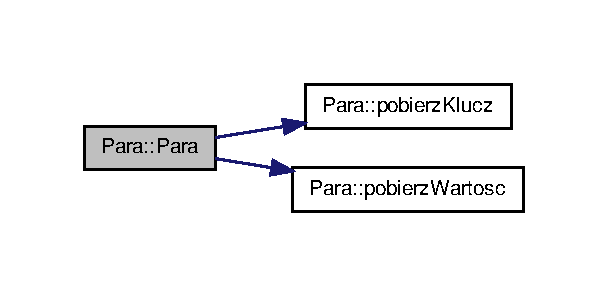
\includegraphics[width=292pt]{class_para_a0229fba16ccbc9e3019d6db3cf9a6d51_cgraph}
\end{center}
\end{figure}




\subsection{\-Dokumentacja funkcji składowych}
\hypertarget{class_para_a2290aed234696b309e979ae269e142ff}{\index{\-Para@{\-Para}!pobierz\-Klucz@{pobierz\-Klucz}}
\index{pobierz\-Klucz@{pobierz\-Klucz}!Para@{\-Para}}
\subsubsection[{pobierz\-Klucz}]{\setlength{\rightskip}{0pt plus 5cm}template$<$typename K , typename W $>$ \-K \& {\bf \-Para}$<$ \-K, \-W $>$\-::{\bf pobierz\-Klucz} (
\begin{DoxyParamCaption}
\item[{void}]{}
\end{DoxyParamCaption}
) const}}\label{class_para_a2290aed234696b309e979ae269e142ff}


\-Funkcja pobierz\-Klucz. \-Zwraca klucz. 



\-Oto graf wywoływań tej funkcji\-:\nopagebreak
\begin{figure}[H]
\begin{center}
\leavevmode
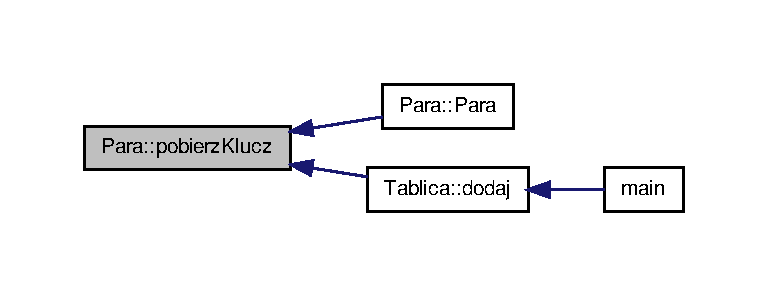
\includegraphics[width=350pt]{class_para_a2290aed234696b309e979ae269e142ff_icgraph}
\end{center}
\end{figure}


\hypertarget{class_para_a3081579446074d32816e0299743208ca}{\index{\-Para@{\-Para}!pobierz\-Wartosc@{pobierz\-Wartosc}}
\index{pobierz\-Wartosc@{pobierz\-Wartosc}!Para@{\-Para}}
\subsubsection[{pobierz\-Wartosc}]{\setlength{\rightskip}{0pt plus 5cm}template$<$typename K , typename W $>$ \-W \& {\bf \-Para}$<$ \-K, \-W $>$\-::{\bf pobierz\-Wartosc} (
\begin{DoxyParamCaption}
\item[{void}]{}
\end{DoxyParamCaption}
) const}}\label{class_para_a3081579446074d32816e0299743208ca}


\-Funkcja pobierz\-Wartosc. \-Zwraca wartosc. 



\-Oto graf wywoływań tej funkcji\-:\nopagebreak
\begin{figure}[H]
\begin{center}
\leavevmode
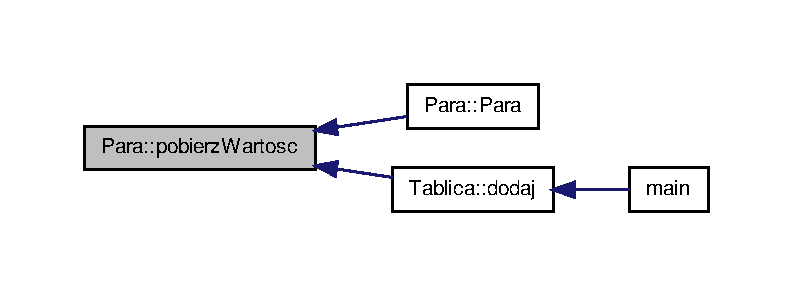
\includegraphics[width=350pt]{class_para_a3081579446074d32816e0299743208ca_icgraph}
\end{center}
\end{figure}


\hypertarget{class_para_a5582293e44ba99f062dcb9fa8e99beaf}{\index{\-Para@{\-Para}!ustaw\-Klucz@{ustaw\-Klucz}}
\index{ustaw\-Klucz@{ustaw\-Klucz}!Para@{\-Para}}
\subsubsection[{ustaw\-Klucz}]{\setlength{\rightskip}{0pt plus 5cm}template$<$typename K , typename W $>$ void {\bf \-Para}$<$ \-K, \-W $>$\-::{\bf ustaw\-Klucz} (
\begin{DoxyParamCaption}
\item[{\-K}]{klucz}
\end{DoxyParamCaption}
)}}\label{class_para_a5582293e44ba99f062dcb9fa8e99beaf}


\-Funkcja ustaw\-Klucz. \-Ustawia klucz. 



\-Oto graf wywoływań tej funkcji\-:\nopagebreak
\begin{figure}[H]
\begin{center}
\leavevmode
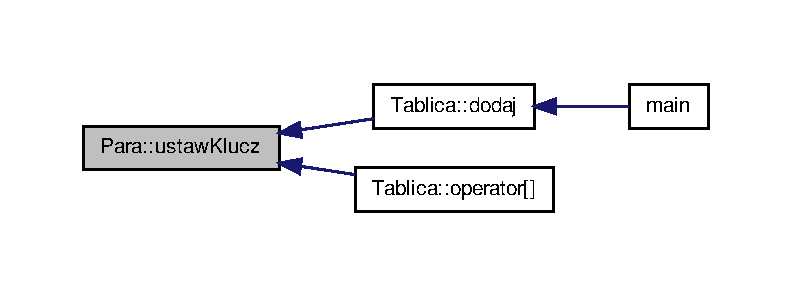
\includegraphics[width=350pt]{class_para_a5582293e44ba99f062dcb9fa8e99beaf_icgraph}
\end{center}
\end{figure}


\hypertarget{class_para_aee0473cc5204fb4b86b2698c0bd7d150}{\index{\-Para@{\-Para}!ustaw\-Wartosc@{ustaw\-Wartosc}}
\index{ustaw\-Wartosc@{ustaw\-Wartosc}!Para@{\-Para}}
\subsubsection[{ustaw\-Wartosc}]{\setlength{\rightskip}{0pt plus 5cm}template$<$typename K , typename W $>$ void {\bf \-Para}$<$ \-K, \-W $>$\-::{\bf ustaw\-Wartosc} (
\begin{DoxyParamCaption}
\item[{\-W}]{wartosc}
\end{DoxyParamCaption}
)}}\label{class_para_aee0473cc5204fb4b86b2698c0bd7d150}


\-Funkcja ustaw\-Wartosc. \-Ustawia wartosc. 



\subsection{\-Dokumentacja atrybutów składowych}
\hypertarget{class_para_a1cf136d1d7c4c7fca4662a04276d744a}{\index{\-Para@{\-Para}!klucz@{klucz}}
\index{klucz@{klucz}!Para@{\-Para}}
\subsubsection[{klucz}]{\setlength{\rightskip}{0pt plus 5cm}template$<$typename \-K, typename \-W$>$ \-K$\ast$ {\bf \-Para}$<$ \-K, \-W $>$\-::{\bf klucz}\hspace{0.3cm}{\ttfamily  \mbox{[}private\mbox{]}}}}\label{class_para_a1cf136d1d7c4c7fca4662a04276d744a}


\-Definicja zmiennej klucz. 

\hypertarget{class_para_a942bf7c31ea059ed0cfe1ac41bb21d6b}{\index{\-Para@{\-Para}!wartosc@{wartosc}}
\index{wartosc@{wartosc}!Para@{\-Para}}
\subsubsection[{wartosc}]{\setlength{\rightskip}{0pt plus 5cm}template$<$typename \-K, typename \-W$>$ \-W$\ast$ {\bf \-Para}$<$ \-K, \-W $>$\-::{\bf wartosc}\hspace{0.3cm}{\ttfamily  \mbox{[}private\mbox{]}}}}\label{class_para_a942bf7c31ea059ed0cfe1ac41bb21d6b}


\-Definicja zmiennej wartosc. 



\-Dokumentacja dla tej klasy została wygenerowana z pliku\-:\begin{DoxyCompactItemize}
\item 
\hyperlink{_para_8h}{\-Para.\-h}\end{DoxyCompactItemize}

\hypertarget{class_tablica}{\section{\-Dokumentacja szablonu klasy \-Tablica$<$ \-K, \-W $>$}
\label{class_tablica}\index{\-Tablica$<$ K, W $>$@{\-Tablica$<$ K, W $>$}}
}


{\ttfamily \#include $<$\-Tablica.\-h$>$}

\subsection*{\-Metody publiczne}
\begin{DoxyCompactItemize}
\item 
\hyperlink{class_tablica_ae1408ffc077347605b61ea0899ddebed}{\-Tablica} (int \hyperlink{class_tablica_a40b3c86ceb2ec860b9d19ce0e866b406}{rozmiar})
\item 
\hyperlink{class_tablica_aabb6e01e32fd2d32ddcfba2c10b9ec5e}{$\sim$\-Tablica} ()
\item 
void \hyperlink{class_tablica_aebb17d3366e37c8b4852df08eae2a1de}{dodaj} (\hyperlink{class_para}{\-Para}$<$ \-K, \-W $>$ \&para)
\item 
void \hyperlink{class_tablica_a061a219dd25c6696940f40226d99a99d}{usun} (\-K klucz)
\item 
\-W \hyperlink{class_tablica_a6de46e3062f16d78c4cb2cf18c9b0de1}{pobierz\-Wartosc} (\-K klucz)
\item 
bool \hyperlink{class_tablica_a19d8da0353d73517375cf6b2984f9d5c}{czypusta} ()
\item 
int \hyperlink{class_tablica_aabc40f316cf398a07e3035b1c4adc256}{size} ()
\item 
\-W \& \hyperlink{class_tablica_a7f5a2d2ebe594ec98dd38dfbbb83497d}{operator\mbox{[}$\,$\mbox{]}} (\-K klucz)
\end{DoxyCompactItemize}
\subsection*{\-Metody prywatne}
\begin{DoxyCompactItemize}
\item 
int \hyperlink{class_tablica_a8fd66d75553eb44aa043f917fd9317dc}{haszstring} (\-K key)
\end{DoxyCompactItemize}
\subsection*{\-Atrybuty prywatne}
\begin{DoxyCompactItemize}
\item 
\hyperlink{class_para}{\-Para}$<$ \-K, \-W $>$ $\ast$$\ast$ \hyperlink{class_tablica_a0d6b03ac0a2b996d4096038ef9315e9a}{tablica}
\item 
int \hyperlink{class_tablica_a603b571fcc0d29b757bfd5fe27d0fadc}{liczba\-Elementow}
\item 
int \hyperlink{class_tablica_a40b3c86ceb2ec860b9d19ce0e866b406}{rozmiar}
\end{DoxyCompactItemize}


\subsection{\-Opis szczegółowy}
\subsubsection*{template$<$typename \-K, typename \-W$>$class Tablica$<$ K, W $>$}

\-Modeluje pojecie tablicy z haszowaniem. \-Klasa modeluje pojecie tablicy z haszowaniem. \-Jej atrybutami sa pola\-: klucz i wartosc. 

\subsection{\-Dokumentacja konstruktora i destruktora}
\hypertarget{class_tablica_ae1408ffc077347605b61ea0899ddebed}{\index{\-Tablica@{\-Tablica}!\-Tablica@{\-Tablica}}
\index{\-Tablica@{\-Tablica}!Tablica@{\-Tablica}}
\subsubsection[{\-Tablica}]{\setlength{\rightskip}{0pt plus 5cm}template$<$typename K , typename W $>$ {\bf \-Tablica}$<$ \-K, \-W $>$\-::{\bf \-Tablica} (
\begin{DoxyParamCaption}
\item[{int}]{rozmiar}
\end{DoxyParamCaption}
)}}\label{class_tablica_ae1408ffc077347605b61ea0899ddebed}


\-Konstruktor klasy \hyperlink{class_tablica}{\-Tablica}. \-Jego argumentem jest maksymalny rozmiar tablicy. 

\hypertarget{class_tablica_aabb6e01e32fd2d32ddcfba2c10b9ec5e}{\index{\-Tablica@{\-Tablica}!$\sim$\-Tablica@{$\sim$\-Tablica}}
\index{$\sim$\-Tablica@{$\sim$\-Tablica}!Tablica@{\-Tablica}}
\subsubsection[{$\sim$\-Tablica}]{\setlength{\rightskip}{0pt plus 5cm}template$<$typename K , typename W $>$ {\bf \-Tablica}$<$ \-K, \-W $>$\-::$\sim${\bf \-Tablica} (
\begin{DoxyParamCaption}
{}
\end{DoxyParamCaption}
)}}\label{class_tablica_aabb6e01e32fd2d32ddcfba2c10b9ec5e}


\-Destruktor klasy \hyperlink{class_tablica}{\-Tablica}. \-Czysci pamiec. 



\subsection{\-Dokumentacja funkcji składowych}
\hypertarget{class_tablica_a19d8da0353d73517375cf6b2984f9d5c}{\index{\-Tablica@{\-Tablica}!czypusta@{czypusta}}
\index{czypusta@{czypusta}!Tablica@{\-Tablica}}
\subsubsection[{czypusta}]{\setlength{\rightskip}{0pt plus 5cm}template$<$typename \-K, typename \-W$>$ bool {\bf \-Tablica}$<$ \-K, \-W $>$\-::{\bf czypusta} (
\begin{DoxyParamCaption}
{}
\end{DoxyParamCaption}
)\hspace{0.3cm}{\ttfamily  \mbox{[}inline\mbox{]}}}}\label{class_tablica_a19d8da0353d73517375cf6b2984f9d5c}


\-Sprawdza zapelnienie tablicy. 

\begin{DoxyReturn}{\-Zwraca}
zwraca prawde, gdy tablica jest pusta 
\end{DoxyReturn}
\hypertarget{class_tablica_aebb17d3366e37c8b4852df08eae2a1de}{\index{\-Tablica@{\-Tablica}!dodaj@{dodaj}}
\index{dodaj@{dodaj}!Tablica@{\-Tablica}}
\subsubsection[{dodaj}]{\setlength{\rightskip}{0pt plus 5cm}template$<$typename K , typename W $>$ void {\bf \-Tablica}$<$ \-K, \-W $>$\-::{\bf dodaj} (
\begin{DoxyParamCaption}
\item[{{\bf \-Para}$<$ \-K, \-W $>$ \&}]{para}
\end{DoxyParamCaption}
)}}\label{class_tablica_aebb17d3366e37c8b4852df08eae2a1de}


\-Funkcja dodaj. \-Dodaje krotke do tablicy. 



\-Oto graf wywołań dla tej funkcji\-:\nopagebreak
\begin{figure}[H]
\begin{center}
\leavevmode
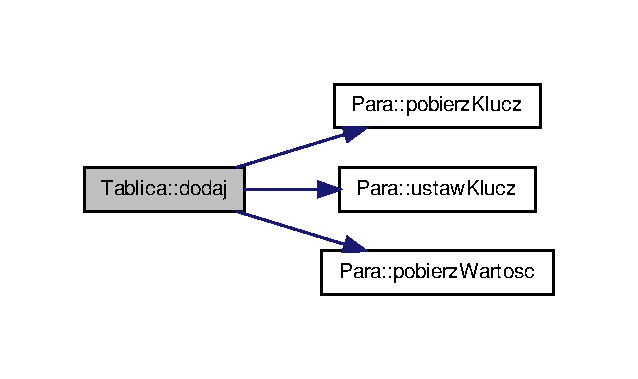
\includegraphics[width=306pt]{class_tablica_aebb17d3366e37c8b4852df08eae2a1de_cgraph}
\end{center}
\end{figure}




\-Oto graf wywoływań tej funkcji\-:\nopagebreak
\begin{figure}[H]
\begin{center}
\leavevmode
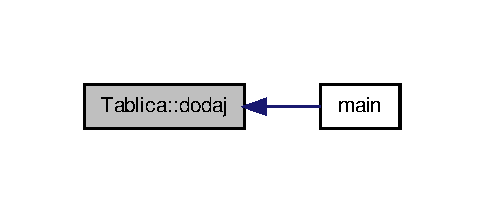
\includegraphics[width=232pt]{class_tablica_aebb17d3366e37c8b4852df08eae2a1de_icgraph}
\end{center}
\end{figure}


\hypertarget{class_tablica_a8fd66d75553eb44aa043f917fd9317dc}{\index{\-Tablica@{\-Tablica}!haszstring@{haszstring}}
\index{haszstring@{haszstring}!Tablica@{\-Tablica}}
\subsubsection[{haszstring}]{\setlength{\rightskip}{0pt plus 5cm}template$<$typename K , typename W $>$ int {\bf \-Tablica}$<$ \-K, \-W $>$\-::{\bf haszstring} (
\begin{DoxyParamCaption}
\item[{\-K}]{key}
\end{DoxyParamCaption}
)\hspace{0.3cm}{\ttfamily  \mbox{[}private\mbox{]}}}}\label{class_tablica_a8fd66d75553eb44aa043f917fd9317dc}


\-Funkcja haszujaca dla obiektow typu string. 

\hypertarget{class_tablica_a7f5a2d2ebe594ec98dd38dfbbb83497d}{\index{\-Tablica@{\-Tablica}!operator\mbox{[}$\,$\mbox{]}@{operator[]}}
\index{operator\mbox{[}$\,$\mbox{]}@{operator[]}!Tablica@{\-Tablica}}
\subsubsection[{operator[]}]{\setlength{\rightskip}{0pt plus 5cm}template$<$typename K , typename W $>$ \-W \& {\bf \-Tablica}$<$ \-K, \-W $>$\-::operator\mbox{[}$\,$\mbox{]} (
\begin{DoxyParamCaption}
\item[{\-K}]{klucz}
\end{DoxyParamCaption}
)}}\label{class_tablica_a7f5a2d2ebe594ec98dd38dfbbb83497d}


\-Przeciazenie operatora indeksujacego. 

\begin{DoxyReturn}{\-Zwraca}
\-Zwraca wartosc. 
\end{DoxyReturn}


\-Oto graf wywołań dla tej funkcji\-:\nopagebreak
\begin{figure}[H]
\begin{center}
\leavevmode
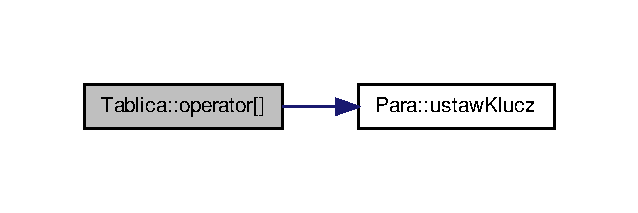
\includegraphics[width=306pt]{class_tablica_a7f5a2d2ebe594ec98dd38dfbbb83497d_cgraph}
\end{center}
\end{figure}


\hypertarget{class_tablica_a6de46e3062f16d78c4cb2cf18c9b0de1}{\index{\-Tablica@{\-Tablica}!pobierz\-Wartosc@{pobierz\-Wartosc}}
\index{pobierz\-Wartosc@{pobierz\-Wartosc}!Tablica@{\-Tablica}}
\subsubsection[{pobierz\-Wartosc}]{\setlength{\rightskip}{0pt plus 5cm}template$<$typename K , typename W $>$ \-W {\bf \-Tablica}$<$ \-K, \-W $>$\-::{\bf pobierz\-Wartosc} (
\begin{DoxyParamCaption}
\item[{\-K}]{klucz}
\end{DoxyParamCaption}
)}}\label{class_tablica_a6de46e3062f16d78c4cb2cf18c9b0de1}


\-Funkcja pobierz\-Wartosc. 

\begin{DoxyReturn}{\-Zwraca}
\-Zwraca wartosc przypisana do danego klucza. 
\end{DoxyReturn}


\-Oto graf wywoływań tej funkcji\-:\nopagebreak
\begin{figure}[H]
\begin{center}
\leavevmode
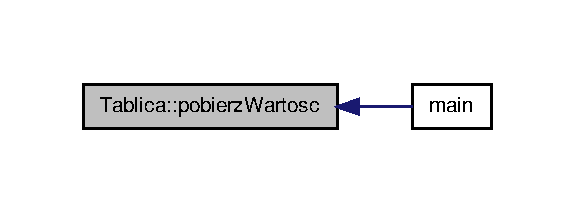
\includegraphics[width=276pt]{class_tablica_a6de46e3062f16d78c4cb2cf18c9b0de1_icgraph}
\end{center}
\end{figure}


\hypertarget{class_tablica_aabc40f316cf398a07e3035b1c4adc256}{\index{\-Tablica@{\-Tablica}!size@{size}}
\index{size@{size}!Tablica@{\-Tablica}}
\subsubsection[{size}]{\setlength{\rightskip}{0pt plus 5cm}template$<$typename \-K, typename \-W$>$ int {\bf \-Tablica}$<$ \-K, \-W $>$\-::{\bf size} (
\begin{DoxyParamCaption}
{}
\end{DoxyParamCaption}
)\hspace{0.3cm}{\ttfamily  \mbox{[}inline\mbox{]}}}}\label{class_tablica_aabc40f316cf398a07e3035b1c4adc256}


\-Podaje liczbe elementow w tablicy. 

\begin{DoxyReturn}{\-Zwraca}
zwraca liczbe elementow w tablicy. 
\end{DoxyReturn}
\hypertarget{class_tablica_a061a219dd25c6696940f40226d99a99d}{\index{\-Tablica@{\-Tablica}!usun@{usun}}
\index{usun@{usun}!Tablica@{\-Tablica}}
\subsubsection[{usun}]{\setlength{\rightskip}{0pt plus 5cm}template$<$typename K , typename W $>$ void {\bf \-Tablica}$<$ \-K, \-W $>$\-::{\bf usun} (
\begin{DoxyParamCaption}
\item[{\-K}]{klucz}
\end{DoxyParamCaption}
)}}\label{class_tablica_a061a219dd25c6696940f40226d99a99d}


\-Funkcja usun. \-Usuwa krotke o podanym kluczu. 



\-Oto graf wywoływań tej funkcji\-:\nopagebreak
\begin{figure}[H]
\begin{center}
\leavevmode
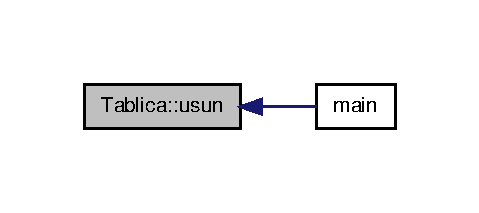
\includegraphics[width=230pt]{class_tablica_a061a219dd25c6696940f40226d99a99d_icgraph}
\end{center}
\end{figure}




\subsection{\-Dokumentacja atrybutów składowych}
\hypertarget{class_tablica_a603b571fcc0d29b757bfd5fe27d0fadc}{\index{\-Tablica@{\-Tablica}!liczba\-Elementow@{liczba\-Elementow}}
\index{liczba\-Elementow@{liczba\-Elementow}!Tablica@{\-Tablica}}
\subsubsection[{liczba\-Elementow}]{\setlength{\rightskip}{0pt plus 5cm}template$<$typename \-K, typename \-W$>$ int {\bf \-Tablica}$<$ \-K, \-W $>$\-::{\bf liczba\-Elementow}\hspace{0.3cm}{\ttfamily  \mbox{[}private\mbox{]}}}}\label{class_tablica_a603b571fcc0d29b757bfd5fe27d0fadc}


\-Obecna liczba elementow w tablicy. 

\hypertarget{class_tablica_a40b3c86ceb2ec860b9d19ce0e866b406}{\index{\-Tablica@{\-Tablica}!rozmiar@{rozmiar}}
\index{rozmiar@{rozmiar}!Tablica@{\-Tablica}}
\subsubsection[{rozmiar}]{\setlength{\rightskip}{0pt plus 5cm}template$<$typename \-K, typename \-W$>$ int {\bf \-Tablica}$<$ \-K, \-W $>$\-::{\bf rozmiar}\hspace{0.3cm}{\ttfamily  \mbox{[}private\mbox{]}}}}\label{class_tablica_a40b3c86ceb2ec860b9d19ce0e866b406}


\-Maksymalna liczba elementow w tablicy. 

\hypertarget{class_tablica_a0d6b03ac0a2b996d4096038ef9315e9a}{\index{\-Tablica@{\-Tablica}!tablica@{tablica}}
\index{tablica@{tablica}!Tablica@{\-Tablica}}
\subsubsection[{tablica}]{\setlength{\rightskip}{0pt plus 5cm}template$<$typename \-K, typename \-W$>$ {\bf \-Para}$<$\-K,\-W$>$$\ast$$\ast$ {\bf \-Tablica}$<$ \-K, \-W $>$\-::{\bf tablica}\hspace{0.3cm}{\ttfamily  \mbox{[}private\mbox{]}}}}\label{class_tablica_a0d6b03ac0a2b996d4096038ef9315e9a}


\hyperlink{class_tablica}{\-Tablica} par. 



\-Dokumentacja dla tej klasy została wygenerowana z pliku\-:\begin{DoxyCompactItemize}
\item 
\hyperlink{_tablica_8h}{\-Tablica.\-h}\end{DoxyCompactItemize}

\hypertarget{class_wezel}{\section{\-Dokumentacja szablonu klasy \-Wezel$<$ \-K, \-W $>$}
\label{class_wezel}\index{\-Wezel$<$ K, W $>$@{\-Wezel$<$ K, W $>$}}
}


{\ttfamily \#include $<$\-Wezel.\-h$>$}



\-Diagram współpracy dla \-Wezel$<$ \-K, \-W $>$\-:\nopagebreak
\begin{figure}[H]
\begin{center}
\leavevmode
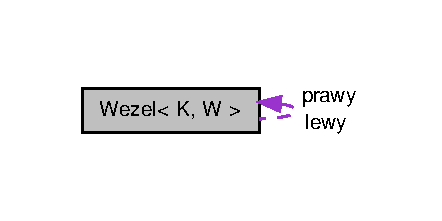
\includegraphics[width=212pt]{class_wezel__coll__graph}
\end{center}
\end{figure}
\subsection*{\-Metody publiczne}
\begin{DoxyCompactItemize}
\item 
\hyperlink{class_wezel_a53d3ba4254af71bdf944878ce0f69552}{\-Wezel} (\hyperlink{class_para}{\-Para}$<$ \-K, \-W $>$ \hyperlink{class_wezel_a4ce56c464874565cc027ce9660cf8e25}{para})
\item 
\hyperlink{class_wezel_a0cd481c65e68ade2fd5a1f142c6995a5}{\-Wezel} ()
\item 
\hyperlink{class_wezel_a55c98fea43ceb7c06e2317754df6626a}{$\sim$\-Wezel} ()
\item 
\hyperlink{class_wezel_a32218370d2423ff2e42f65926c74c767}{\-Wezel} (const \hyperlink{class_wezel}{\-Wezel} \&wezel)
\item 
void \hyperlink{class_wezel_acfc2260875484193f734f2eeed617062}{osieroc} ()
\end{DoxyCompactItemize}
\subsection*{\-Atrybuty publiczne}
\begin{DoxyCompactItemize}
\item 
\hyperlink{class_para}{\-Para}$<$ \-K, \-W $>$ $\ast$ \hyperlink{class_wezel_a4ce56c464874565cc027ce9660cf8e25}{para}
\item 
\hyperlink{class_wezel}{\-Wezel} $\ast$ \hyperlink{class_wezel_ae58a8e38a89e571a26afa5e2ca93a1f5}{lewy}
\item 
\hyperlink{class_wezel}{\-Wezel} $\ast$ \hyperlink{class_wezel_a5b54943e3c95535fbf59be020808e359}{prawy}
\end{DoxyCompactItemize}


\subsection{\-Opis szczegółowy}
\subsubsection*{template$<$typename \-K, typename \-W$>$class Wezel$<$ K, W $>$}

\-Modeluje pojecie wezla. \-Jego atrybutem jest klasa \hyperlink{class_para}{\-Para}. 

\subsection{\-Dokumentacja konstruktora i destruktora}
\hypertarget{class_wezel_a53d3ba4254af71bdf944878ce0f69552}{\index{\-Wezel@{\-Wezel}!\-Wezel@{\-Wezel}}
\index{\-Wezel@{\-Wezel}!Wezel@{\-Wezel}}
\subsubsection[{\-Wezel}]{\setlength{\rightskip}{0pt plus 5cm}template$<$typename K , typename W $>$ {\bf \-Wezel}$<$ \-K, \-W $>$\-::{\bf \-Wezel} (
\begin{DoxyParamCaption}
\item[{{\bf \-Para}$<$ \-K, \-W $>$}]{para}
\end{DoxyParamCaption}
)}}\label{class_wezel_a53d3ba4254af71bdf944878ce0f69552}


\-Konstruktor klasy \hyperlink{class_wezel}{\-Wezel}. \-Jego argumentem jest klasa \hyperlink{class_para}{\-Para}. 

\hypertarget{class_wezel_a0cd481c65e68ade2fd5a1f142c6995a5}{\index{\-Wezel@{\-Wezel}!\-Wezel@{\-Wezel}}
\index{\-Wezel@{\-Wezel}!Wezel@{\-Wezel}}
\subsubsection[{\-Wezel}]{\setlength{\rightskip}{0pt plus 5cm}template$<$typename \-K, typename \-W$>$ {\bf \-Wezel}$<$ \-K, \-W $>$\-::{\bf \-Wezel} (
\begin{DoxyParamCaption}
{}
\end{DoxyParamCaption}
)\hspace{0.3cm}{\ttfamily  \mbox{[}inline\mbox{]}}}}\label{class_wezel_a0cd481c65e68ade2fd5a1f142c6995a5}
\hypertarget{class_wezel_a55c98fea43ceb7c06e2317754df6626a}{\index{\-Wezel@{\-Wezel}!$\sim$\-Wezel@{$\sim$\-Wezel}}
\index{$\sim$\-Wezel@{$\sim$\-Wezel}!Wezel@{\-Wezel}}
\subsubsection[{$\sim$\-Wezel}]{\setlength{\rightskip}{0pt plus 5cm}template$<$typename K , typename W $>$ {\bf \-Wezel}$<$ \-K, \-W $>$\-::$\sim${\bf \-Wezel} (
\begin{DoxyParamCaption}
{}
\end{DoxyParamCaption}
)}}\label{class_wezel_a55c98fea43ceb7c06e2317754df6626a}


\-Destruktor klasy \hyperlink{class_wezel}{\-Wezel}. \-Czysci pamiec po obiekcie. 

\hypertarget{class_wezel_a32218370d2423ff2e42f65926c74c767}{\index{\-Wezel@{\-Wezel}!\-Wezel@{\-Wezel}}
\index{\-Wezel@{\-Wezel}!Wezel@{\-Wezel}}
\subsubsection[{\-Wezel}]{\setlength{\rightskip}{0pt plus 5cm}template$<$typename K , typename W $>$ {\bf \-Wezel}$<$ \-K, \-W $>$\-::{\bf \-Wezel} (
\begin{DoxyParamCaption}
\item[{const {\bf \-Wezel}$<$ \-K, \-W $>$ \&}]{wezel}
\end{DoxyParamCaption}
)}}\label{class_wezel_a32218370d2423ff2e42f65926c74c767}


\-Konstruktor kopiujacy klasy \hyperlink{class_wezel}{\-Wezel}. \-Kopiuje obiekt. 



\subsection{\-Dokumentacja funkcji składowych}
\hypertarget{class_wezel_acfc2260875484193f734f2eeed617062}{\index{\-Wezel@{\-Wezel}!osieroc@{osieroc}}
\index{osieroc@{osieroc}!Wezel@{\-Wezel}}
\subsubsection[{osieroc}]{\setlength{\rightskip}{0pt plus 5cm}template$<$typename K , typename W $>$ void {\bf \-Wezel}$<$ \-K, \-W $>$\-::{\bf osieroc} (
\begin{DoxyParamCaption}
{}
\end{DoxyParamCaption}
)}}\label{class_wezel_acfc2260875484193f734f2eeed617062}


\-Funkcja osieroc. \-Ustawia wskazniki na dzieci na \-N\-U\-L\-L. 



\subsection{\-Dokumentacja atrybutów składowych}
\hypertarget{class_wezel_ae58a8e38a89e571a26afa5e2ca93a1f5}{\index{\-Wezel@{\-Wezel}!lewy@{lewy}}
\index{lewy@{lewy}!Wezel@{\-Wezel}}
\subsubsection[{lewy}]{\setlength{\rightskip}{0pt plus 5cm}template$<$typename \-K, typename \-W$>$ {\bf \-Wezel}$\ast$ {\bf \-Wezel}$<$ \-K, \-W $>$\-::{\bf lewy}}}\label{class_wezel_ae58a8e38a89e571a26afa5e2ca93a1f5}


\-Definicja zmiennej lewy. 

\hypertarget{class_wezel_a4ce56c464874565cc027ce9660cf8e25}{\index{\-Wezel@{\-Wezel}!para@{para}}
\index{para@{para}!Wezel@{\-Wezel}}
\subsubsection[{para}]{\setlength{\rightskip}{0pt plus 5cm}template$<$typename \-K, typename \-W$>$ {\bf \-Para}$<$\-K,\-W$>$$\ast$ {\bf \-Wezel}$<$ \-K, \-W $>$\-::{\bf para}}}\label{class_wezel_a4ce56c464874565cc027ce9660cf8e25}


\-Definicja zmiennej para. 

\hypertarget{class_wezel_a5b54943e3c95535fbf59be020808e359}{\index{\-Wezel@{\-Wezel}!prawy@{prawy}}
\index{prawy@{prawy}!Wezel@{\-Wezel}}
\subsubsection[{prawy}]{\setlength{\rightskip}{0pt plus 5cm}template$<$typename \-K, typename \-W$>$ {\bf \-Wezel}$\ast$ {\bf \-Wezel}$<$ \-K, \-W $>$\-::{\bf prawy}}}\label{class_wezel_a5b54943e3c95535fbf59be020808e359}


\-Definicja zmiennej prawy. 



\-Dokumentacja dla tej klasy została wygenerowana z pliku\-:\begin{DoxyCompactItemize}
\item 
\hyperlink{_wezel_8h}{\-Wezel.\-h}\end{DoxyCompactItemize}

\chapter{\-Dokumentacja plików}
\hypertarget{_drzewo_8h}{\section{\-Dokumentacja pliku \-Drzewo.\-h}
\label{_drzewo_8h}\index{\-Drzewo.\-h@{\-Drzewo.\-h}}
}
{\ttfamily \#include \char`\"{}\-Wezel.\-h\char`\"{}}\*
{\ttfamily \#include $<$string.\-h$>$}\*
{\ttfamily \#include \char`\"{}\-Para.\-h\char`\"{}}\*
\-Wykres zależności załączania dla \-Drzewo.\-h\-:
\nopagebreak
\begin{figure}[H]
\begin{center}
\leavevmode
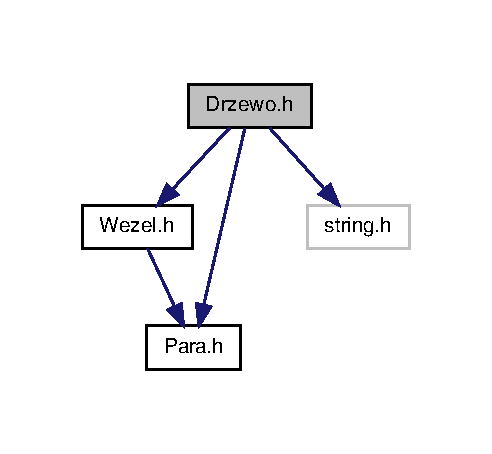
\includegraphics[width=236pt]{_drzewo_8h__incl}
\end{center}
\end{figure}
\-Ten wykres pokazuje, które pliki bezpośrednio lub pośrednio załączają ten plik\-:
\nopagebreak
\begin{figure}[H]
\begin{center}
\leavevmode
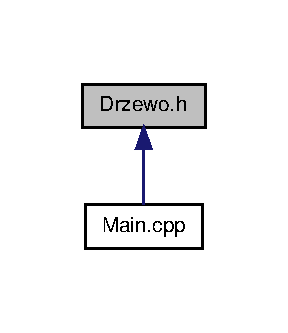
\includegraphics[width=138pt]{_drzewo_8h__dep__incl}
\end{center}
\end{figure}
\subsection*{\-Komponenty}
\begin{DoxyCompactItemize}
\item 
class \hyperlink{class_drzewo}{\-Drzewo$<$ K, W $>$}
\begin{DoxyCompactList}\small\item\em \-Modeluje pojecie drzewa binarnego. \-Jego atrybutem jest klasa \hyperlink{class_wezel}{\-Wezel}. \end{DoxyCompactList}\end{DoxyCompactItemize}


\subsection{\-Opis szczegółowy}
\-Definicja szablonu klasy \hyperlink{class_drzewo}{\-Drzewo} \-Plik zawiera definicje szablonu klasy \hyperlink{class_drzewo}{\-Drzewo}. 
\hypertarget{_main_8cpp}{\section{\-Dokumentacja pliku \-Main.\-cpp}
\label{_main_8cpp}\index{\-Main.\-cpp@{\-Main.\-cpp}}
}
{\ttfamily \#include $<$iostream$>$}\*
{\ttfamily \#include \char`\"{}\-Tablica.\-h\char`\"{}}\*
{\ttfamily \#include \char`\"{}\-Drzewo.\-h\char`\"{}}\*
{\ttfamily \#include $<$time.\-h$>$}\*
\-Wykres zależności załączania dla \-Main.\-cpp\-:
\nopagebreak
\begin{figure}[H]
\begin{center}
\leavevmode
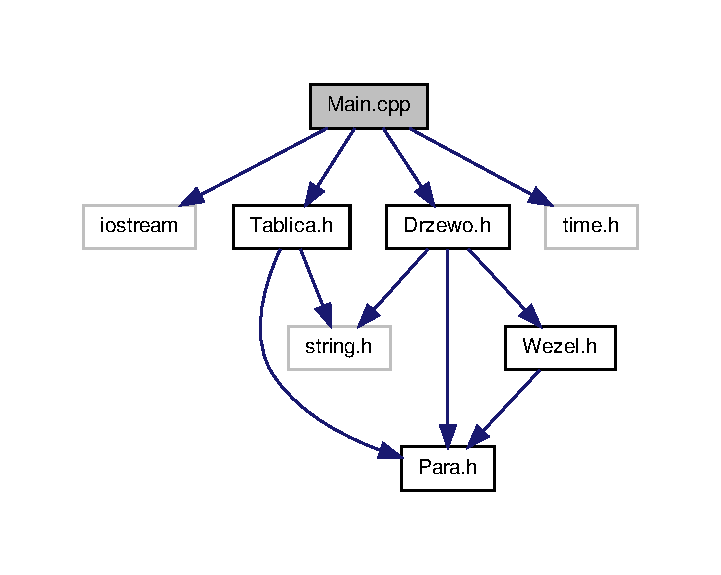
\includegraphics[width=346pt]{_main_8cpp__incl}
\end{center}
\end{figure}
\subsection*{\-Funkcje}
\begin{DoxyCompactItemize}
\item 
string \hyperlink{_main_8cpp_ab922b9da141e16dbcc98dda9fa91687c}{gen\-\_\-random} (const int len)
\item 
int \hyperlink{_main_8cpp_ae66f6b31b5ad750f1fe042a706a4e3d4}{main} ()
\end{DoxyCompactItemize}


\subsection{\-Dokumentacja funkcji}
\hypertarget{_main_8cpp_ab922b9da141e16dbcc98dda9fa91687c}{\index{\-Main.\-cpp@{\-Main.\-cpp}!gen\-\_\-random@{gen\-\_\-random}}
\index{gen\-\_\-random@{gen\-\_\-random}!Main.cpp@{\-Main.\-cpp}}
\subsubsection[{gen\-\_\-random}]{\setlength{\rightskip}{0pt plus 5cm}string {\bf gen\-\_\-random} (
\begin{DoxyParamCaption}
\item[{const int}]{len}
\end{DoxyParamCaption}
)}}\label{_main_8cpp_ab922b9da141e16dbcc98dda9fa91687c}


\-Oto graf wywoływań tej funkcji\-:\nopagebreak
\begin{figure}[H]
\begin{center}
\leavevmode
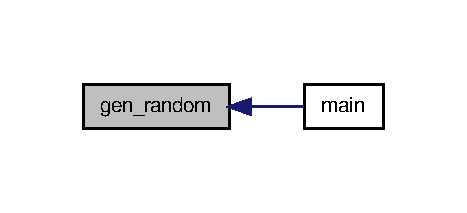
\includegraphics[width=224pt]{_main_8cpp_ab922b9da141e16dbcc98dda9fa91687c_icgraph}
\end{center}
\end{figure}


\hypertarget{_main_8cpp_ae66f6b31b5ad750f1fe042a706a4e3d4}{\index{\-Main.\-cpp@{\-Main.\-cpp}!main@{main}}
\index{main@{main}!Main.cpp@{\-Main.\-cpp}}
\subsubsection[{main}]{\setlength{\rightskip}{0pt plus 5cm}int {\bf main} (
\begin{DoxyParamCaption}
{}
\end{DoxyParamCaption}
)}}\label{_main_8cpp_ae66f6b31b5ad750f1fe042a706a4e3d4}


\-Oto graf wywołań dla tej funkcji\-:
\nopagebreak
\begin{figure}[H]
\begin{center}
\leavevmode
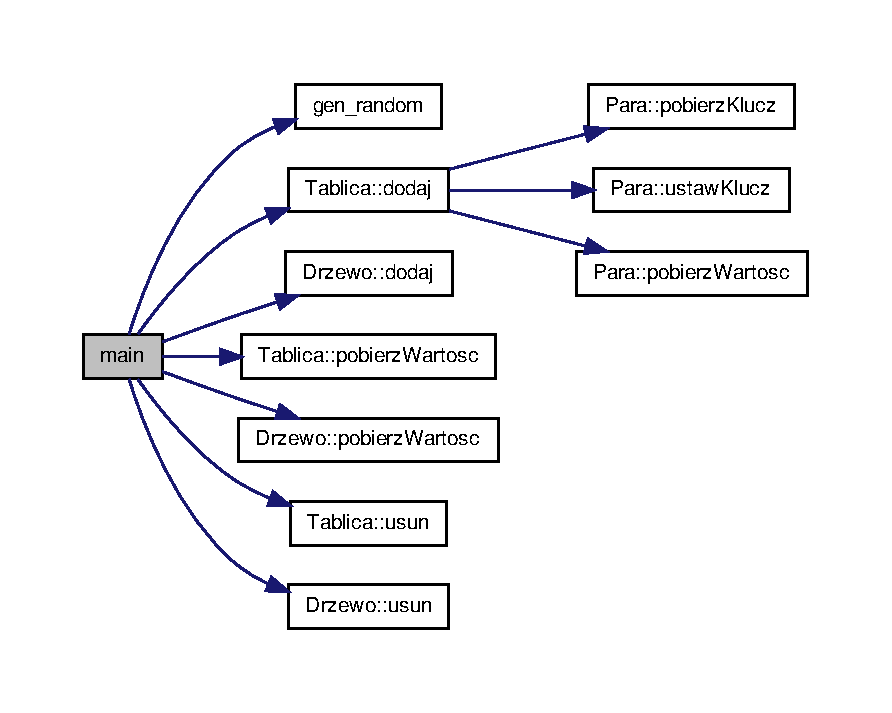
\includegraphics[width=350pt]{_main_8cpp_ae66f6b31b5ad750f1fe042a706a4e3d4_cgraph}
\end{center}
\end{figure}



\hypertarget{_para_8cpp}{\section{\-Dokumentacja pliku \-Para.\-cpp}
\label{_para_8cpp}\index{\-Para.\-cpp@{\-Para.\-cpp}}
}

\hypertarget{_para_8h}{\section{\-Dokumentacja pliku \-Para.\-h}
\label{_para_8h}\index{\-Para.\-h@{\-Para.\-h}}
}
\-Ten wykres pokazuje, które pliki bezpośrednio lub pośrednio załączają ten plik\-:
\nopagebreak
\begin{figure}[H]
\begin{center}
\leavevmode
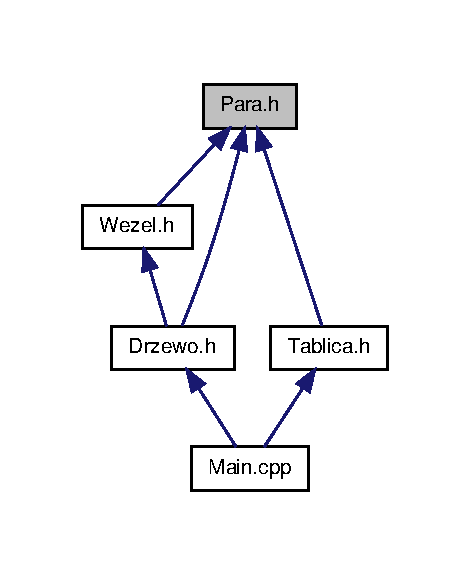
\includegraphics[width=226pt]{_para_8h__dep__incl}
\end{center}
\end{figure}
\subsection*{\-Komponenty}
\begin{DoxyCompactItemize}
\item 
class \hyperlink{class_para}{\-Para$<$ K, W $>$}
\begin{DoxyCompactList}\small\item\em \-Modeluje pojecie pary. \-Jej atrybutem sa pola zawierajace klucz i wartosci. \end{DoxyCompactList}\end{DoxyCompactItemize}


\subsection{\-Opis szczegółowy}
\-Definicja szablonu klasy \hyperlink{class_para}{\-Para} \-Plik zawiera definicje szablonu klasy \hyperlink{class_para}{\-Para}. 
\hypertarget{_tablica_8h}{\section{\-Dokumentacja pliku \-Tablica.\-h}
\label{_tablica_8h}\index{\-Tablica.\-h@{\-Tablica.\-h}}
}
{\ttfamily \#include \char`\"{}\-Para.\-h\char`\"{}}\*
{\ttfamily \#include $<$string.\-h$>$}\*
\-Wykres zależności załączania dla \-Tablica.\-h\-:
\nopagebreak
\begin{figure}[H]
\begin{center}
\leavevmode
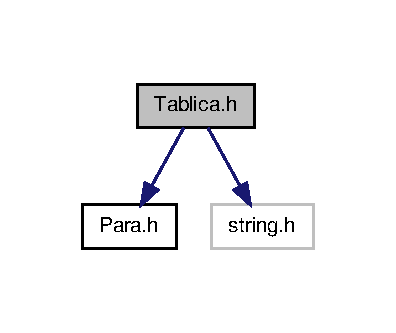
\includegraphics[width=190pt]{_tablica_8h__incl}
\end{center}
\end{figure}
\-Ten wykres pokazuje, które pliki bezpośrednio lub pośrednio załączają ten plik\-:
\nopagebreak
\begin{figure}[H]
\begin{center}
\leavevmode
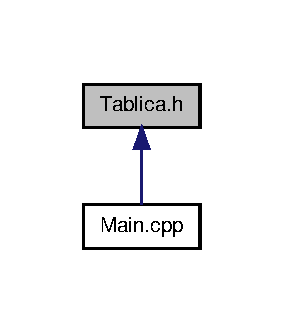
\includegraphics[width=136pt]{_tablica_8h__dep__incl}
\end{center}
\end{figure}
\subsection*{\-Komponenty}
\begin{DoxyCompactItemize}
\item 
class \hyperlink{class_tablica}{\-Tablica$<$ K, W $>$}
\begin{DoxyCompactList}\small\item\em \-Modeluje pojecie tablicy z haszowaniem. \-Klasa modeluje pojecie tablicy z haszowaniem. \-Jej atrybutami sa pola\-: klucz i wartosc. \end{DoxyCompactList}\end{DoxyCompactItemize}


\subsection{\-Opis szczegółowy}
\-Definicja szablonu klasy \-Tablica(tablicab z haszowaniem) \-Plik zawiera definicje szablonu klasy \-Tablica.\-Jest to klasa glowna , ktora wykorzystuje klase \hyperlink{class_para}{\-Para}. 
\hypertarget{_wezel_8h}{\section{\-Dokumentacja pliku \-Wezel.\-h}
\label{_wezel_8h}\index{\-Wezel.\-h@{\-Wezel.\-h}}
}
{\ttfamily \#include \char`\"{}\-Para.\-h\char`\"{}}\*
\-Wykres zależności załączania dla \-Wezel.\-h\-:
\nopagebreak
\begin{figure}[H]
\begin{center}
\leavevmode
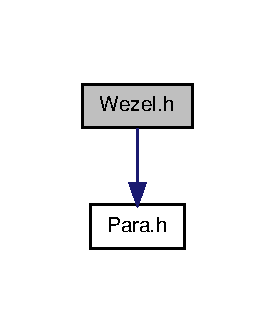
\includegraphics[width=132pt]{_wezel_8h__incl}
\end{center}
\end{figure}
\-Ten wykres pokazuje, które pliki bezpośrednio lub pośrednio załączają ten plik\-:
\nopagebreak
\begin{figure}[H]
\begin{center}
\leavevmode
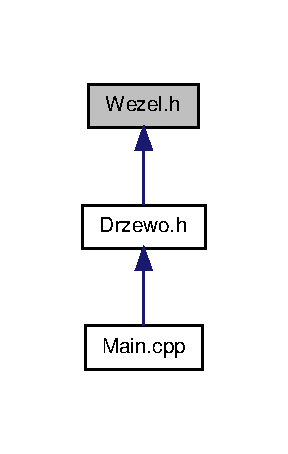
\includegraphics[width=138pt]{_wezel_8h__dep__incl}
\end{center}
\end{figure}
\subsection*{\-Komponenty}
\begin{DoxyCompactItemize}
\item 
class \hyperlink{class_wezel}{\-Wezel$<$ K, W $>$}
\begin{DoxyCompactList}\small\item\em \-Modeluje pojecie wezla. \-Jego atrybutem jest klasa \hyperlink{class_para}{\-Para}. \end{DoxyCompactList}\end{DoxyCompactItemize}


\subsection{\-Opis szczegółowy}
\-Definicja szablonu klasy \hyperlink{class_wezel}{\-Wezel} \-Plik zawiera definicje szablonu klasy \hyperlink{class_wezel}{\-Wezel}. 
\printindex
\end{document}
